\documentclass[10pt, a4paper]{article}

\usepackage[]{graphicx}
\usepackage{subcaption}
\usepackage[]{hyperref}
\usepackage{listings}
\usepackage{color}
\usepackage{amsmath}
\usepackage{ gensymb }
\usepackage{parskip}
\definecolor{red}{rgb}{1,0,0}
\definecolor{green}{rgb}{0,1,0}
\definecolor{codegreen}{rgb}{0,0.6,0}
\definecolor{codegray}{rgb}{0.5,0.5,0.5}
\definecolor{codepurple}{rgb}{0.58,0,0.82}
\definecolor{backcolour}{rgb}{0.95,0.95,0.92}

\lstdefinestyle{mystyle}{
    backgroundcolor=\color{backcolour},   
    commentstyle=\color{blue},
    numberstyle=\tiny\color{codepurple},
    stringstyle=\color{codegreen},
    basicstyle=\footnotesize,
    breakatwhitespace=false,         
    breaklines=true,                 
    captionpos=b,                    
    keepspaces=true,                 
    numbers=left,                    
    numbersep=5pt,                  
    showspaces=false,                
    showstringspaces=false,
    showtabs=false,                  
    tabsize=2
}
 
\lstset{style=mystyle}
\usepackage[utf8]{inputenc}

\lstset{
% 	frame = single,
% 	language = R,
% 	showstringspaces = false,
% 	tabsize = 2,
	otherkeywords = {self},
	keywordstyle = \color{magenta},
	identifierstyle=\color{black},
%	numberstyle = \color{yellow},
	stringstyle=\color{orange},
% 	backgroundcolor=\color{backcolour}
}

\title{Oblig 1 The Traveling Salesman Problem \\
  \hrulefill\small{ INF4490 }\hrulefill}
  
\author{Joseph Knutson \\
\href{https://github.com/mathhat/}{\texttt{github.com/mathhat}}}
  
\begin{document}

\maketitle
\tableofcontents
\clearpage
\section{Exhaustive search}
This section guides you through the code, efficiency and result of the exhaustive search method for the traveling salesman problem.
\subsection{Creating the Code}
Making my Exhaustive Search code began with using the example.py file on the course site which imports the city grid.
From there I followed the advice of the assignment regarding the itertools module's permutations function. Looping over every sequence and summing the distances for each sequence, the final Exhaustive search function looked something like this:
\begin{lstlisting}[language = Python]
  start = time.time()             #start clock
  for sequence in Permutations:   #exhaustive search begins
      dist = 0
      for index in range(cities-1):
	        dist += distances[sequence[index]][sequence[index+1]]
      dist += distances[sequence[cities-1]][sequence[0]]
      if dist < best:             #save shortest distance yet
	        best=dist
	        best_sequence = sequence

  end = time.time()              #end clock
  Time = (end-start)             #sum time
  return(best, best_sequence, Time)
\end{lstlisting}
You can observe on the last line that the function returns the shortest path's distance, the path sequence and the time it took to iterate over all the permutations.
\subsection{Timetables}
The time it takes for the program to run varies with the amount of cities we add. However, it is not sufficiently accurate to measure only once.
Calling the Exhaustive Search function 10 times helped create an approximate time average for its execution time, and I did so for the first 6 to 10 cities in the european\_cities.csv file. 
The result can be seen in figure \ref{fig:time_exhaust}. The code calculating the timeaverages and producing the plot lies in the exhaustive\_time.py file.

\begin{figure}[h!]\centering
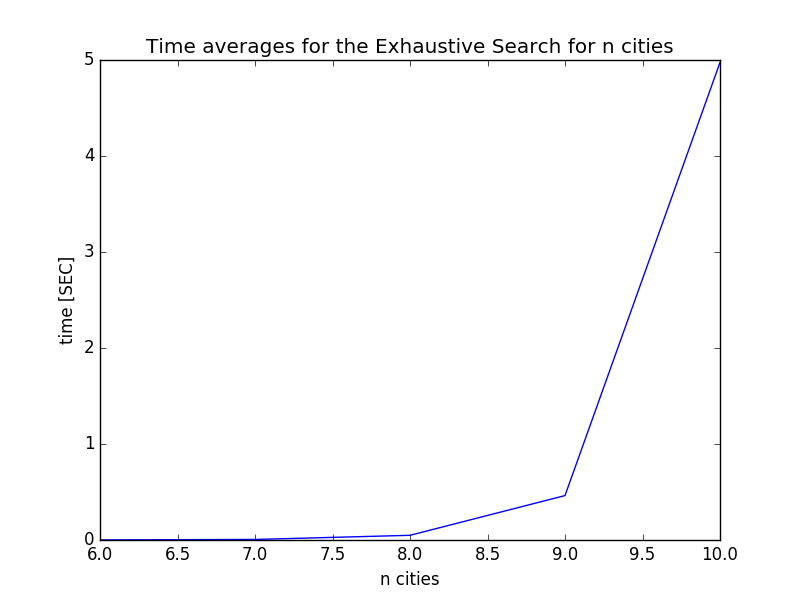
\includegraphics[width = \linewidth]{time_exhaust.png} 
\caption{Time to calculate shortest path as a function of the number of cities.}
\label{fig:time_exhaust}
\end{figure}

If you go into the time\_exhaustive.txt file (created by running exhaustive\_time.py), you can quickly find how long the calculations took (below). Let's use these numbers to predict how long it takes to use Exhaustive Search with 24 cities.
\begin{lstlisting}
Time average for 7 cities = 0.005085 seconds 

Time average for 8 cities = 0.042169 seconds 

Time average for 9 cities = 0.420994 seconds 

Time average for 10 cities = 4.878382 seconds 
\end{lstlisting}
To find out how long simulations of a higher city number will take, we try to make a model based on the amount of flops (+ - * /) that are executed.
The number of permutations for 10 cities are equal to N!$ = 3628800$ and for each permutation (or path) one has to add the distances between each city to calculate the total distance of the path. 
This leaves us with N$*$N!$ = 36288000$ floating point operations (flops). If we divide the amount of flops the program used on the runtime of the program, we get an approximation of how many flops (additions) occur per second:
$$\text{flops\_per\_sec} = \frac{36288000}{4.878382 \text{sec}} = 7438531.87389 \text{flops/sec}$$

This approximation of a constant can give us an idea of how long it takes to run an exhaustive search for a larger amount of cities.
To find the runtime of a larger path with 24 cities, we need to find the amount of flops the program will require (N$*$N!):
$$\text{flops(24 cities)} = 24*24! = 1.4890762\ 10^{25} \text{flops}$$
Now we can calculate the seconds this program will need to finish running (not to mention the insane amount of RAM):
$$\text{runtime of ES for 24 cities} = \frac{1.4890762\ 10^{25} \text{flops}}{\text{flops\_per\_sec}} \approx 63.4\ 10^{9} \text{years} $$
The calculations make it obvious that Exhaustive Search is useless once the amount of cities pass 10.
\subsection{Shortest Path Result}

Our Exhaustive Search function returns not only time, but also the distance, \emph{best}, and the sequence of cities traveled along the shortest path, \emph{sequence}.
\begin{lstlisting}
'Best' = ', 7486.309999999999
'Best sequence = ', (6, 8, 3, 7, 0, 1, 9, 4, 5, 2)

Barcelona, Belgrade, Berlin, Brussels, Bucharest, Budapest, Copenhagen, Dublin, Hamburg, Istanbul
\end{lstlisting}
Above is the result for $n_{cities} = 10$. I've written the cities in alphabetic order. The sequence has translated each city into a number from 0 to 9. 
If we place the 10 cities' names in the order that creates the shortest path, we get: 
\begin{lstlisting}
Copenhagen Hamburg Brussels Dublin Barcelona Belgrade Istanbul Bucharest Budapest Berlin 
\end{lstlisting}
\clearpage
\section{Hillclimber}
This section compares my Hillclimber method with the Exhaustive Search method from the previous assignment. The method I've written is heavily inspired by the course book's (\emph{Machine Learning}) example.
\subsection{Code}
\begin{lstlisting}[language = Python]
swag

\end{lstlisting}

\end{document}